% 2011 年山东卷文科第 10 题：四个选项的函数图象（选项图）。
% 来源 PDF：普通高考/2011/2011山东文.pdf，SHA-256 bf61cf7bb39a3ccfc57735cd2a7ab34387cbfa6bc86a5e7f8246e13292b0e023。
% 原页：第 1 页（A3 三栏）第 2 栏上部，书页码 691。
% 重绘依据：按原页矢量层实测复刻。原点与 2π 刻度相距 35.61pt，故 1 弧度 = 35.61/(2π) = 5.6698pt，
%   下文坐标一律以弧度为单位的无量纲数（4 即 y=4，6.283 即 2π）。
%   四个子图的坐标系同形：x 轴自原点左伸 11.99、右伸 11.36 弧度；y 轴上伸 6.36、下伸 7.00；
%   y 轴在 y=4 处有一个向右的短刻度（长 0.40），x 轴在 x=2π 处有一个向上的短刻度（长 0.40）；
%   文字位置一律取原页字形盒中心（换算成弧度）：y 标签 (-1.13,7.25)、4 标签 (-1.07,3.87)、
%   2π 标签 (6.29,-1.38)、x 标签 (12.05,-0.98)、选项字母 (-14.03,-6.45)；
%   原点 O 的标注位置各图不同且照原页：(A) 在 x 轴上方 (-1.38,1.13)，
%   (B)(C)(D) 都在 x 轴下方约 (-1.37,-1.45)。
%   原页四图都无网格、无虚线。
%   曲线由原页矢量路径数字化反解：(C) 是 y=x/2-2sin x（残差 0.008），即本题正确图象；
%   (A) 是 y=x/2-2cos x（残差 0.0014），在 y 轴上的截距为 -2；
%   (B) 是 y=x-3sin x（残差 0.002），原页只画在 |x|≤4 内；
%   (D) 是原页手绘的干扰曲线，不是解析函数：每侧三段三次贝塞尔，两支关于原点中心对称，
%   振幅随 |x| 增大（x=±1.56 处约 ∓2.14，x=±7 处约 ±4.5），零点在 0、±3.42、±8.8；
%   本图直接使用原页控制点（原页坐标除以 5.6698pt），拓扑与形状照原页。
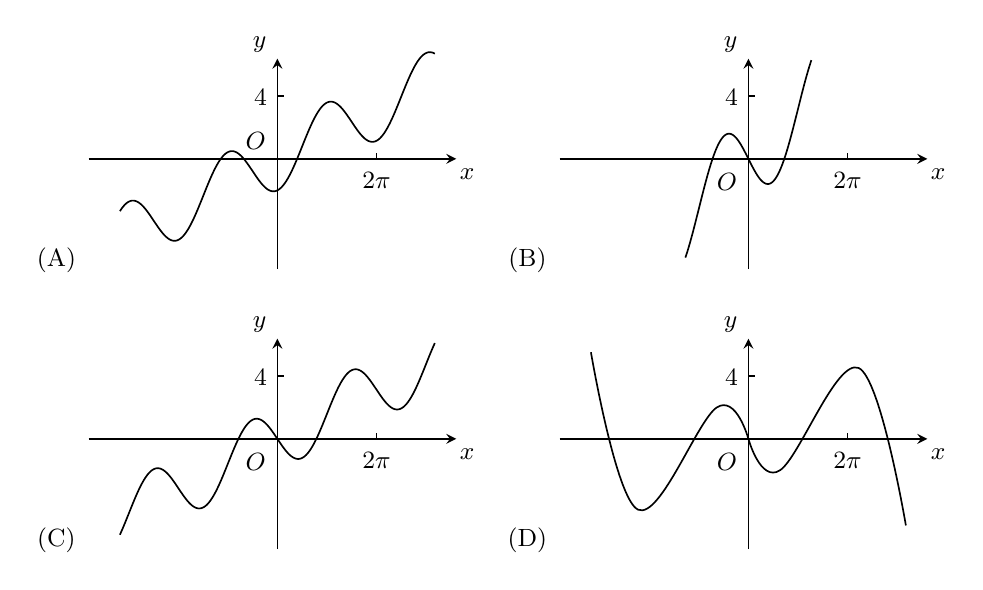
\begin{tikzpicture}[scale=0.20, >=stealth, semithick, font=\small]

  % ===== 四个子图共用的坐标轴（坐标值即原页实测的弧度数；O 的标注各图另放） =====
  \def\axes{
    \draw[->] (-11.99,0) -- (11.36,0);
    \draw[->] (0,-7.00) -- (0,6.36);
    \draw (0,4) -- (0.40,4);
    \draw (6.283,0) -- (6.283,0.40);
    \node at (-1.07,3.87) {$4$};
    \node at (6.29,-1.38) {$2\pi$};
    \node at (12.05,-0.98) {$x$};
    \node at (-1.13,7.25) {$y$};
  }

  % ================= (A) y = x/2 - 2cos x =================
  \begin{scope}
    \axes
    \node at (-1.38,1.13) {$O$};
    \draw[domain=-10:10, samples=300] plot (\x,{\x/2-2*cos(\x r)});
    \node at (-14.03,-6.45) {(A)};
  \end{scope}

  % ================= (B) y = x - 3sin x =================
  \begin{scope}[shift={(29.91,0)}]
    \axes
    \node at (-1.36,-1.45) {$O$};
    \draw[domain=-4:4, samples=200] plot (\x,{\x-3*sin(\x r)});
    \node at (-14.03,-6.45) {(B)};
  \end{scope}

  % ================= (C) y = x/2 - 2sin x =================
  \begin{scope}[shift={(0,-17.78)}]
    \axes
    \node at (-1.38,-1.45) {$O$};
    \draw[domain=-10:10, samples=300] plot (\x,{\x/2-2*sin(\x r)});
    \node at (-14.03,-6.45) {(C)};
  \end{scope}

  % ====== (D) 原页手绘干扰曲线（贝塞尔控制点照原页矢量层） ======
  \begin{scope}[shift={(29.91,-17.78)}]
    \axes
    \node at (-1.36,-1.45) {$O$};
    % 右支：原点 → (2,-2) → (7,4.5) → (10,-5.5)
    \draw (0,0) .. controls (0,0) and (0.767,-2.793) .. (2.000,-2.000)
                .. controls (3.234,-1.207) and (5.590,5.117) .. (7.000,4.500)
                .. controls (8.408,3.883) and (10.000,-5.500) .. (10.000,-5.500);
    % 左支：与右支关于原点中心对称
    \draw (0,0) .. controls (0,0) and (-0.767,2.793) .. (-2.000,2.000)
                .. controls (-3.234,1.207) and (-5.590,-5.117) .. (-7.000,-4.500)
                .. controls (-8.408,-3.883) and (-10.000,5.500) .. (-10.000,5.500);
    \node at (-14.03,-6.45) {(D)};
  \end{scope}

\end{tikzpicture}
